% Scalar instruction entry source: tools/generate_scalar_instruction_catalog.py.
\subsection{\texttt{ADDIW}}
\label{sec:scalar-addiw}
\index{ADDIW@\texttt{ADDIW}}
\begin{sloppypar}\noindent\textbf{Purpose.} Word (32-bit) add-immediate.\end{sloppypar}\smallskip
\noindent\textbf{Syntax.}\par
\begin{lstlisting}[style=ptoscalarcode]
addiw SrcL, uimm, ->RegDst
\end{lstlisting}
\noindent\textbf{Encoding.}\par
\noindent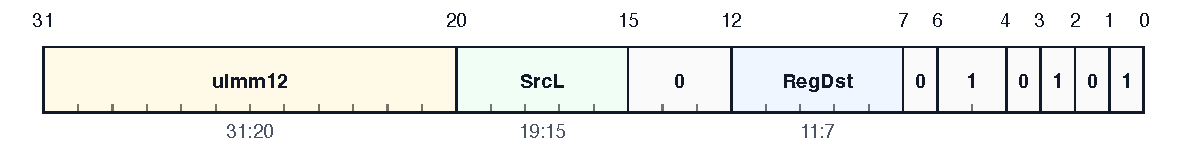
\includegraphics[width=\textwidth]{figs/encoding/scalar_instruction_entries/enc_addiw.pdf}\par\smallskip
\begin{description}[leftmargin=0.18\linewidth,style=nextline]
\item[Format] \texttt{L32} \texttt{32-bit} scalar word.
\item[Pattern] \texttt{.................000.....0110101}.
\end{description}
\noindent\textbf{Classification.}\par
\begin{description}[leftmargin=0.18\linewidth,style=nextline]
\item[Category] Integer ALU and Bit-Manipulation.
\item[Family] Arithmetic Operation 32bit.
\item[Execution class] \texttt{ALU}; uop\_kind=ALU.
\end{description}
\noindent\textbf{Operand fields.}\par
\begin{description}[leftmargin=0.18\linewidth,style=nextline]
\item[\texttt{RegDst}] Bits \texttt{11:7 (5b)}. 5-bit scalar destination register written by this instruction; X0 is hardwired to zero, so writes to X0 are ignored.
\item[\texttt{SrcL}] Bits \texttt{19:15 (5b)}. 5-bit scalar source register used as the left input operand.
\item[\texttt{uimm12}] Bits \texttt{31:20 (12b)}. 12-bit unsigned immediate operand consumed directly by the operation.
\end{description}
\noindent\textbf{Operation.}\par
\begin{lstlisting}[style=ptoscalarcode]
lhs = Read(SrcL)[31:0]
rhs = ZeroExtend(uimm)
result32 = lhs + rhs
Write(RegDst, SignExtend32(result32))
\end{lstlisting}
\Needspace{0.08\textheight}
